\documentclass{article}
\usepackage{mystyle}
\begin{document}
\maketitle

\author{}
\date{}

\textbf{REMOTE ACCESS -TUTORIAL}

\textbf{X2GO \& MobaXterm, Public Key Authentication and .bashrc
Settings}

\begin{enumerate}
\def\labelenumi{\Alph{enumi}.}
\item
  \textbf{X2Go Installation}
\end{enumerate}

\begin{enumerate}
\def\labelenumi{\arabic{enumi}.}
\item
  X2Go is program used to run graphical applications on our Linux
  machines remotely. This uses a different technology from remote X,
  which results in better performance, especially when not on campus.
  This also allows for suspending and resuming sessions and programs,
  while they continue to run. This allows the use of long-running
  graphical applications \cite{Cai2014}.
\item
  The X2Go Client software is already installed on all lab computers.
  For your personal computers, download the X2Go client for your
  operating system:

  \begin{enumerate}
  \def\labelenumii{\arabic{enumii}.}
  \item
    macOS -
    \url{http://code.x2go.org/releases/X2GoClient_latest_macosx.dmg}
  \item
    Windows -
    \url{http://code.x2go.org/releases/X2GoClient_latest_mswin32-setup.exe}
  \end{enumerate}
\item
  On macOS, mount the dmg file (your browser may do this for you after
  download) and drag the x2goclient application to your Applications
  folder. On Windows, double-click the downloaded setup file and follow
  the instructions in the wizard to install the software.
\end{enumerate}

\begin{enumerate}
\def\labelenumi{\Alph{enumi}.}
\setcounter{enumi}{1}
\item
  \textbf{X2Go Configuration}
\end{enumerate}

\begin{enumerate}
\def\labelenumi{\arabic{enumi}.}
\setcounter{enumi}{3}
\item
  When you first run the X2Go client, you will be presented with a
  "\emph{\textbf{New session}}" dialog. You should fill this in with
  this information:
\item
  Session tab

  \begin{enumerate}
  \def\labelenumii{\arabic{enumii}.}
  \item
    Session name - Any name you'd like to identify the session to
    yourself - if you're connecting to
    \emph{\textbf{i80labpc04.ira.uka.de}}, you might just want this to
    be " \emph{\textbf{i80labpc04}}"
  \item
    Host - Full name of the server you're connecting to, e.g.
    \emph{\textbf{i80labpc04.ira.uka.de}}
  \item
    All of our compute machines have the X2Go server installed
  \item
    Login -- Your user ID e.g. ``\emph{\textbf{asip04}}'' (be careful to
    use lower case)
  \item
    Session type - Select XFCE (this is the only supported session type)
    - see below for of session types.
  \end{enumerate}
\end{enumerate}

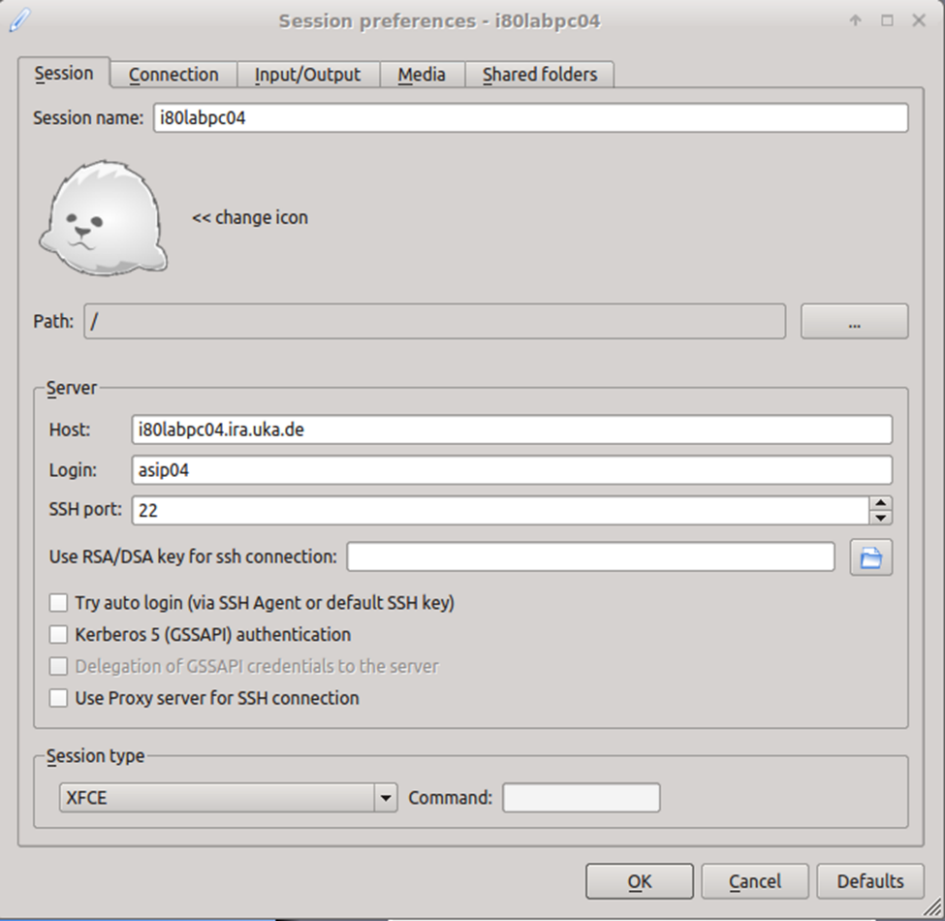
\includegraphics[width=4.28968in,height=4.17836in]{images/media/image1.png}

Figure 1: Session Tab

\begin{enumerate}
\def\labelenumi{\arabic{enumi}.}
\setcounter{enumi}{5}
\item
  Connection tab

  \begin{enumerate}
  \def\labelenumii{\arabic{enumii}.}
  \item
    Connection speed - Set the connection speed you will most often use
    for this connection
  \item
    The default ADSL is fine for most connections, but if you are on
    campus, you will get better graphics performance if you choose LAN
  \end{enumerate}
\end{enumerate}

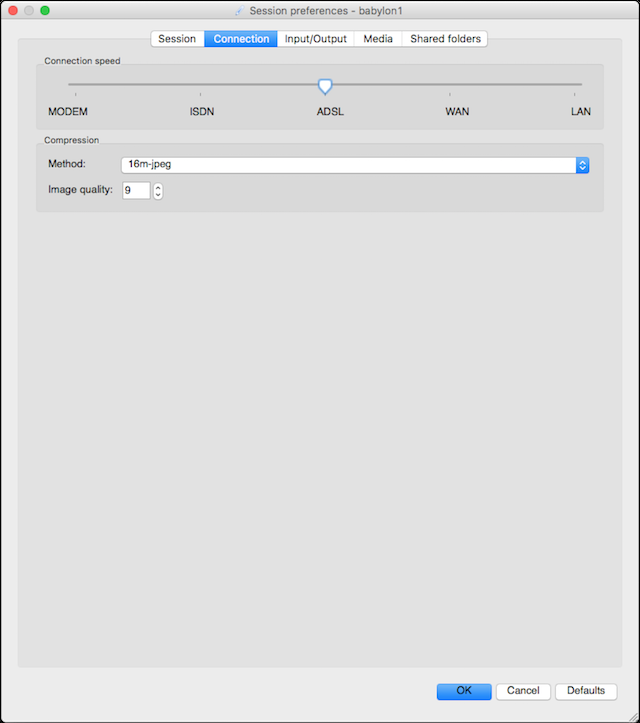
\includegraphics[width=4.66535in,height=5.27165in]{images/media/image2.png}

Figure 2: Connection Tab

\begin{enumerate}
\def\labelenumi{\arabic{enumi}.}
\setcounter{enumi}{6}
\item
  Input/output tab

  \begin{enumerate}
  \def\labelenumii{\arabic{enumii}.}
  \item
    Display - select whether you want to run full screen or at a
    specific resolution
  \end{enumerate}
\item
  Media

  \begin{enumerate}
  \def\labelenumii{\arabic{enumii}.}
  \item
    Client side printing support - be sure to uncheck this box or you
    may get errors when starting the session
  \end{enumerate}
\end{enumerate}

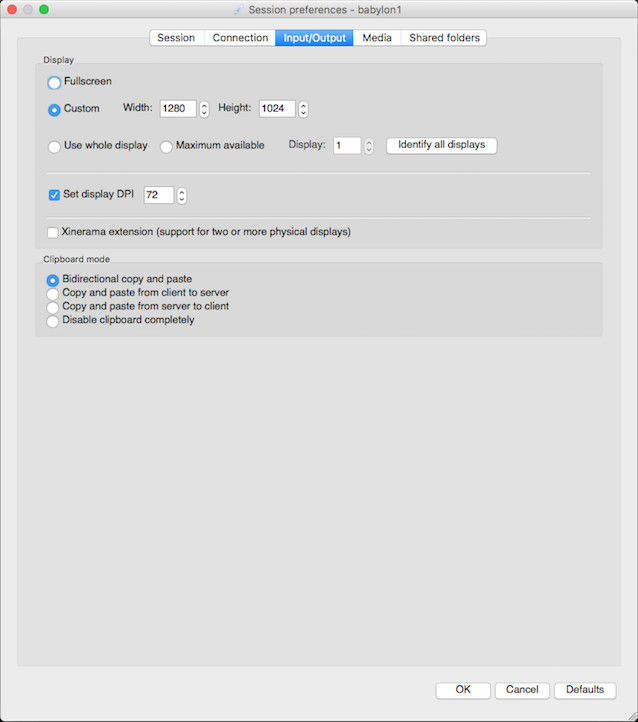
\includegraphics[width=4.00394in,height=4.5315in]{images/media/image3.png}

Figure 3: Input/output Tab

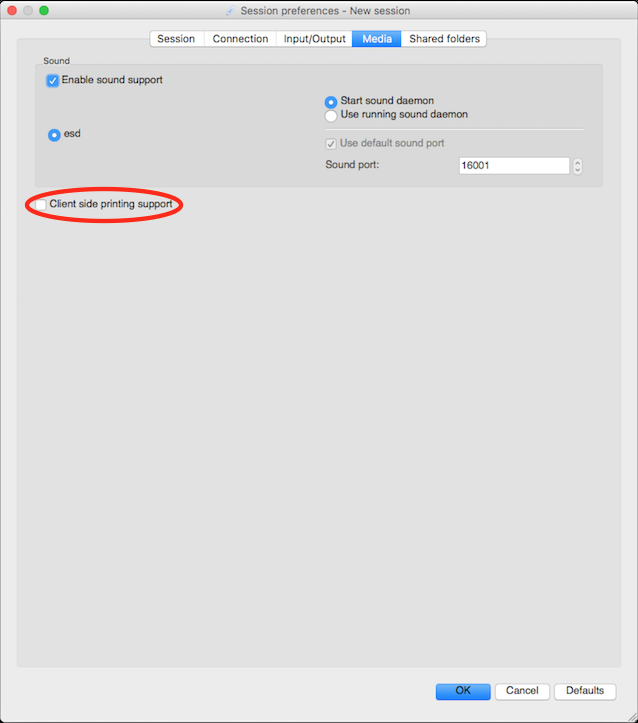
\includegraphics[width=4.00394in,height=4.5315in]{images/media/image4.png}

Figure 4: Media Tab

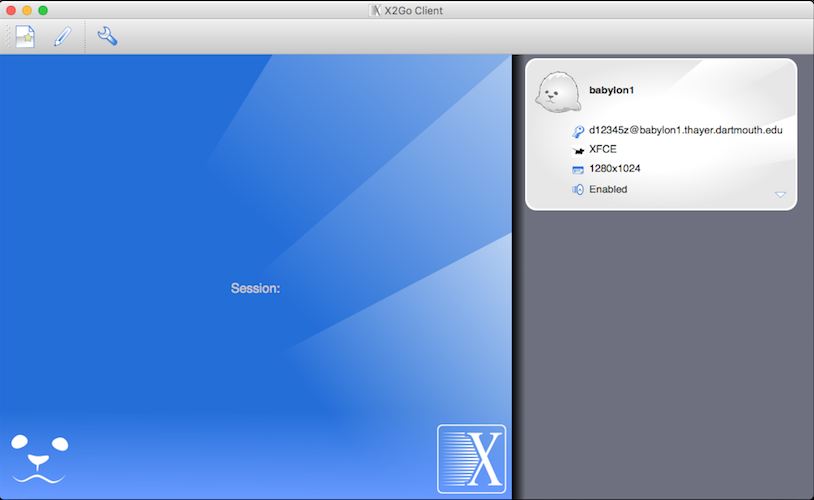
\includegraphics[width=5.50787in,height=3.38189in]{images/media/image5.png}

Figure 5: Main Client Screen

\begin{enumerate}
\def\labelenumi{\Alph{enumi}.}
\setcounter{enumi}{2}
\item
  \textbf{X2Go Session Types}
\end{enumerate}

\begin{enumerate}
\def\labelenumi{\arabic{enumi}.}
\setcounter{enumi}{8}
\item
  The session types that we support are:

  \begin{enumerate}
  \def\labelenumii{\arabic{enumii}.}
  \item
    XFCE (recommended) - This is a low-power window manager that is the
    only one supported in the current version of Ubuntu
  \item
    Published applications - This allows you to run one or more
    applications directly, rather than a full desktop session. See below
    for how to run published applications
  \end{enumerate}
\end{enumerate}

\begin{enumerate}
\def\labelenumi{\Alph{enumi}.}
\setcounter{enumi}{3}
\item
  \textbf{X2Go Connecting}
\end{enumerate}

\begin{enumerate}
\def\labelenumi{\arabic{enumi}.}
\setcounter{enumi}{9}
\item
  To start the session, click on it and provide your password where
  prompted
\end{enumerate}

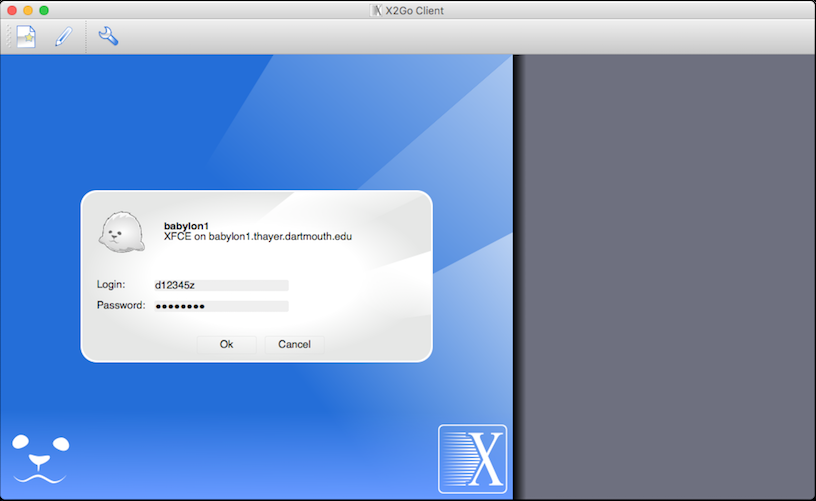
\includegraphics[width=5.50787in,height=3.38189in]{images/media/image6.png}

Figure 6: Login Screen

\begin{enumerate}
\def\labelenumi{\arabic{enumi}.}
\setcounter{enumi}{10}
\item
  After you click OK, it will connect to the server and start your
  session. Watch the Status line to see what's happening. Once the
  status is "running," your session should launch.
\item
  When you first connect to a particular server, you may get a dialog
  box asking you to accept the host key. Click Yes to accept it:
\end{enumerate}

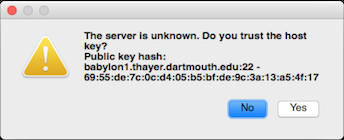
\includegraphics[width=3.58289in,height=1.45815in]{images/media/image7.png}

Figure 7: Host Key Authentication

\begin{enumerate}
\def\labelenumi{\arabic{enumi}.}
\setcounter{enumi}{12}
\item
  To suspend a session, click the suspend button:
\end{enumerate}

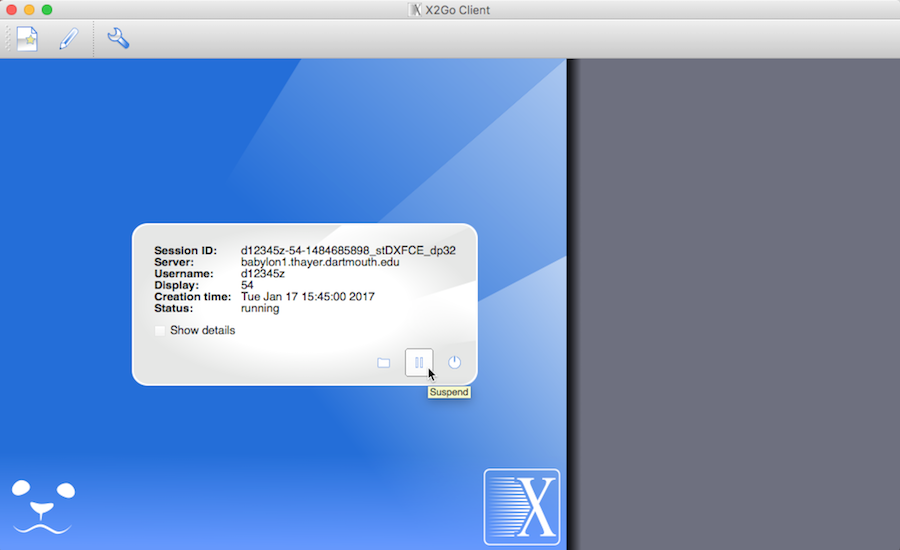
\includegraphics[width=6.08268in,height=3.71654in]{images/media/image8.png}

Figure 8: Suspending a Session

\begin{enumerate}
\def\labelenumi{\arabic{enumi}.}
\setcounter{enumi}{13}
\item
  To terminate, either log out of your session or click the terminate
  button:
\end{enumerate}

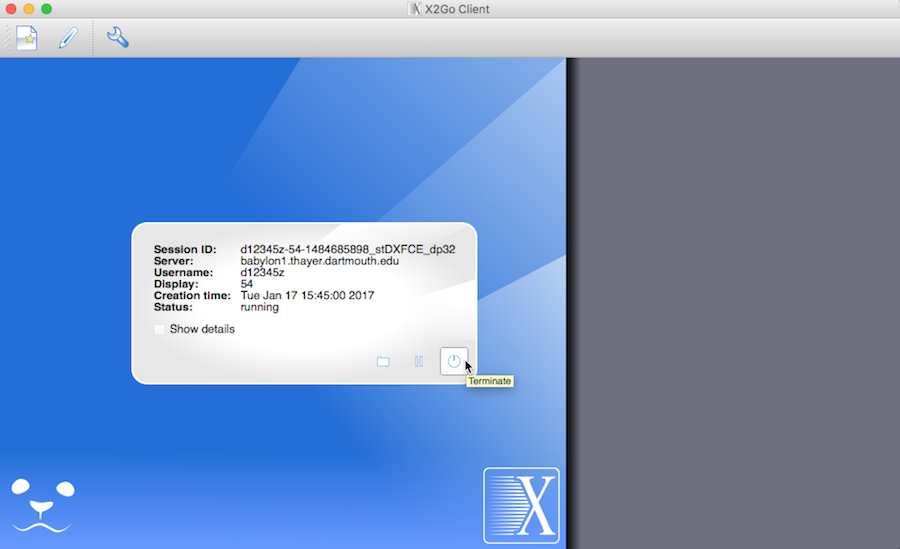
\includegraphics[width=6.26806in,height=3.82311in]{images/media/image9.png}

Figure 9: Terminating a Session

\begin{enumerate}
\def\labelenumi{\Alph{enumi}.}
\setcounter{enumi}{4}
\item
  \textbf{X2Go Resuming}
\end{enumerate}

\begin{enumerate}
\def\labelenumi{\arabic{enumi}.}
\setcounter{enumi}{14}
\item
  If you have a single session open on a particular server and you
  reconnect with the same client, it will automatically re-connect to
  your session.
\item
  If you are connecting from a different client or have multiple
  sessions on the same server, you'll be presented a list to either
  resume an existing session or create a new one:
\end{enumerate}

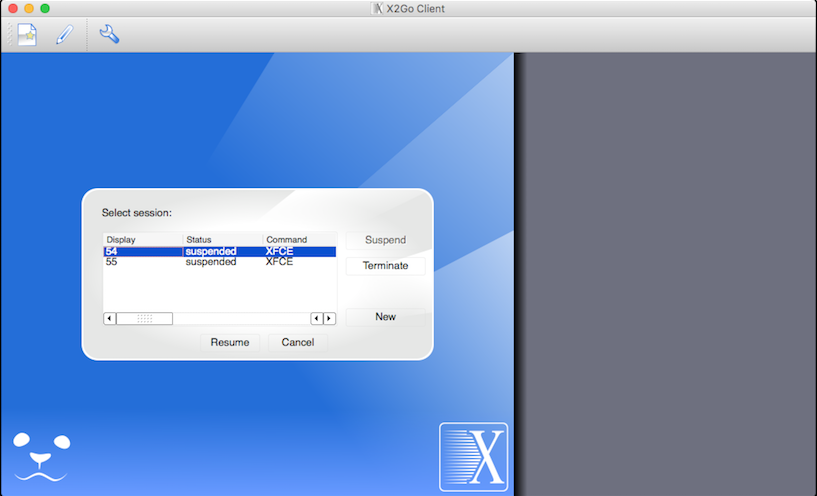
\includegraphics[width=6.26806in,height=3.8057in]{images/media/image10.png}

Figure 10: Resuming a Session

\begin{enumerate}
\def\labelenumi{\Alph{enumi}.}
\setcounter{enumi}{5}
\item
  \textbf{X2Go Published Applications}
\end{enumerate}

\begin{enumerate}
\def\labelenumi{\arabic{enumi}.}
\setcounter{enumi}{16}
\item
  If you choose the "Published Applications" session, after you connect
  the Status will change to running, but it will appear that nothing has
  happened. To choose an application, click the "Applications" button:
\end{enumerate}

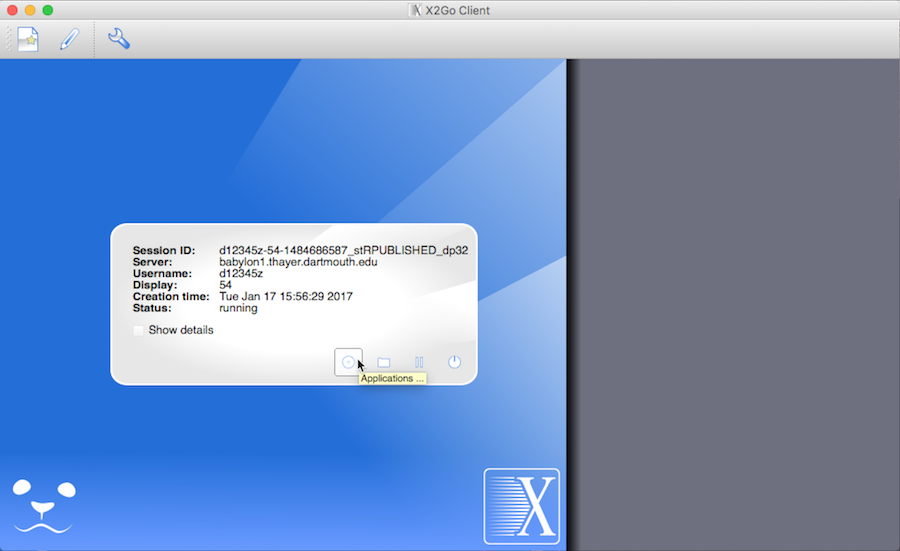
\includegraphics[width=6.26806in,height=3.83718in]{images/media/image11.png}

Figure 11: Published Applications

\begin{enumerate}
\def\labelenumi{\arabic{enumi}.}
\setcounter{enumi}{17}
\item
  This will then bring up a dialog from which you can choose an
  application to run. All Thayer-specific applications are interspersed
  under the "Other" section:
\end{enumerate}

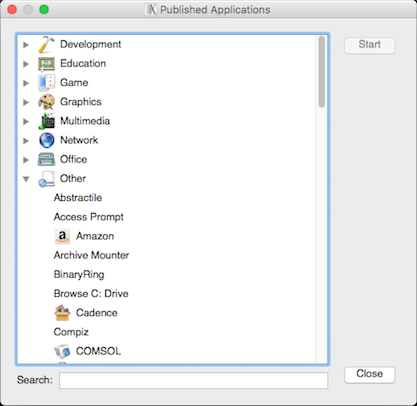
\includegraphics[width=4.07153in,height=3.96413in]{images/media/image12.png}

Figure 12: Applications

\begin{enumerate}
\def\labelenumi{\arabic{enumi}.}
\setcounter{enumi}{18}
\item
  When you click "Start," be patient. This dialog does not go away and
  some programs may take several seconds to start up. Clicking Start
  more than once will launch multiple instances of the same app.
\item
  Fonts for Windows
\item
  When using the X2Go client on Windows, there may be some older
  programs (e.g. Cadence) where fonts do not show up properly. Symptoms
  you may see are either blocky, illegible fonts or instances where
  fonts disappear because they are white on a white background. If you
  experience any of these, you can install a font package that should
  eliminate most of these issues. Keep in mind that this is only needed
  if you are running the X2Go client on Windows.
\item
  First, if you haven't already, follow the instructions at Thayer
  Shares Connecting to connect to Thayer Shares. Navigate to the Courses
  share (P:), and go to the software\textbackslash x2go folder. In this
  folder, double-click the vcxsrv\_fonts.exe file to install the fonts.
  Depending on your security settings, you may need to drag this file to
  your local computer before double-clicking on it.
\item
  Other Settings
\item
  If you are using a Mac and need to use the Alt key within remote
  sessions, you need to change the X11 preferences. Run XQuartz directly
  from within Applications-\textgreater Utilities. Then, select the
  X11-\textgreater Preferences... menu item, select the Input tab, and
  check the box next to "Option keys send Alt\_L and Alt\_R." Close the
  preferences window and quit X11. Then, restart X2Go and when you log
  into a remote session, the option key (also labeled alt on most Mac
  keyboards) will send the Alt key to the remote side.
\end{enumerate}

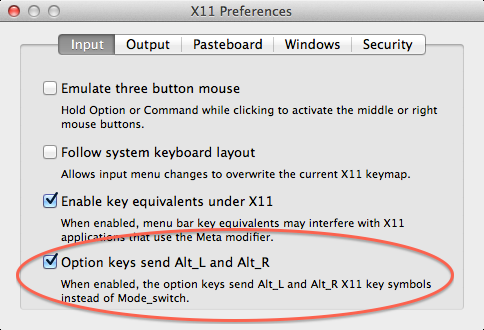
\includegraphics[width=3.78346in,height=2.57874in]{images/media/image13.png}

Figure 13: X11 Preferences

\textbf{\hfill\break
}

\textbf{MobaXterm CLIENT -TUTORIAL}

\begin{enumerate}
\def\labelenumi{\Alph{enumi}.}
\setcounter{enumi}{6}
\item
  \textbf{MobaXterm Installation}
\end{enumerate}

\begin{enumerate}
\def\labelenumi{\arabic{enumi}.}
\item
  Download MobaXterm from
  \url{https://mobaxterm.mobatek.net/download.html}
\item
  Install it with default settings.
\end{enumerate}

\begin{enumerate}
\def\labelenumi{\Alph{enumi}.}
\setcounter{enumi}{7}
\item
  \textbf{MobaXterm Configuration}
\end{enumerate}

\begin{enumerate}
\def\labelenumi{\arabic{enumi}.}
\setcounter{enumi}{2}
\item
  Click on "Sessions" and then on "SSH".
\end{enumerate}

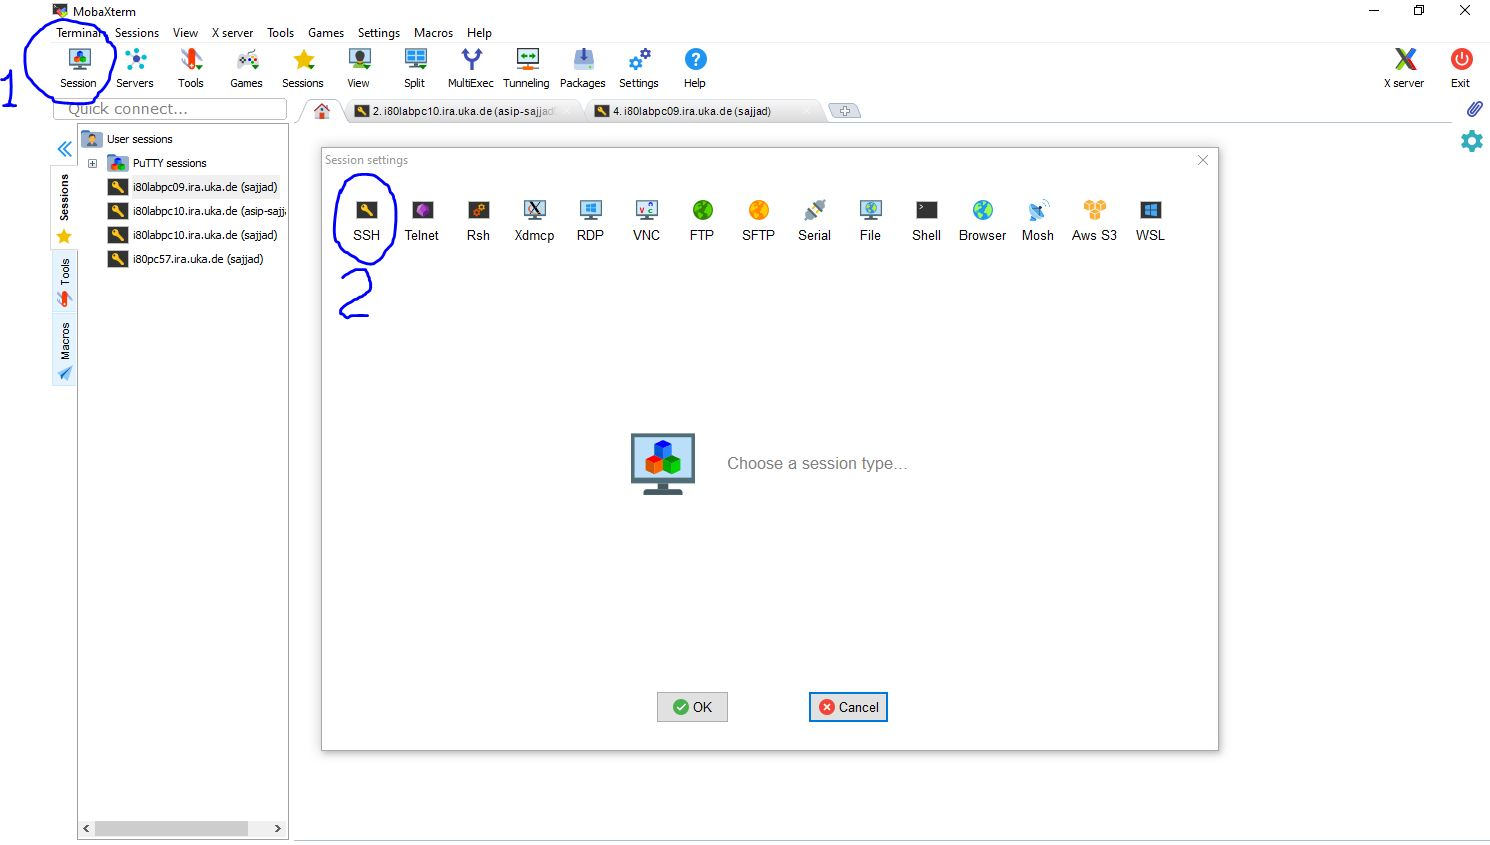
\includegraphics[width=5.73515in,height=3.25226in]{images/media/image14.JPG}

Figure 14: SSH Session

\begin{enumerate}
\def\labelenumi{\arabic{enumi}.}
\setcounter{enumi}{3}
\item
  In the new windows "Session settings", enter \textbf{Remote host} as
  ``\emph{i80labpcXX.ira.uka.de}'', tick the box "\textbf{Specify user
  name}" and then enter your user name as ``\emph{asip-abcdnn}''.
\end{enumerate}

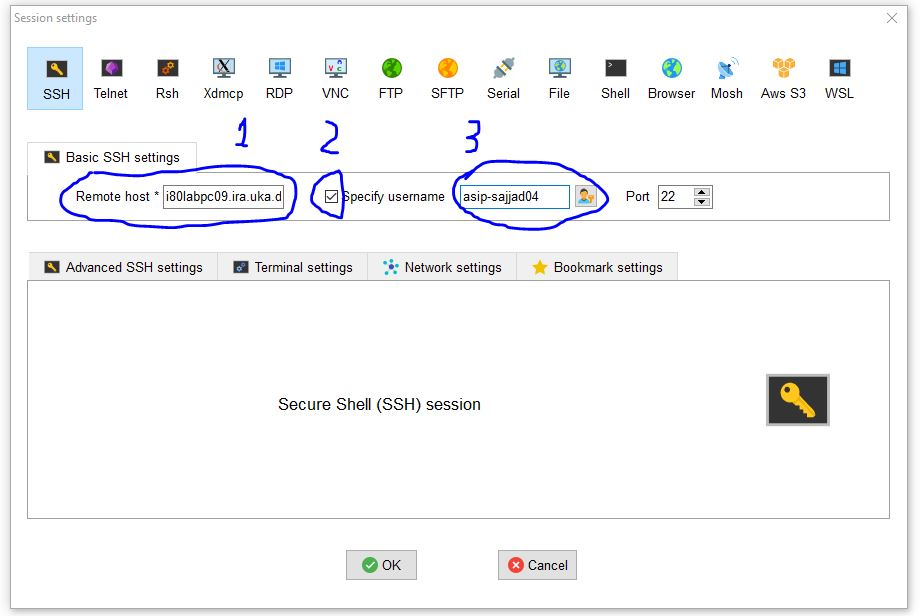
\includegraphics[width=5.53861in,height=3.70864in]{images/media/image15.JPG}

Figure 15: Session Settings

\begin{enumerate}
\def\labelenumi{\arabic{enumi}.}
\setcounter{enumi}{4}
\item
  Press OK. It will ask for the user password.
\item
  Enter your password and press Enter.
\end{enumerate}

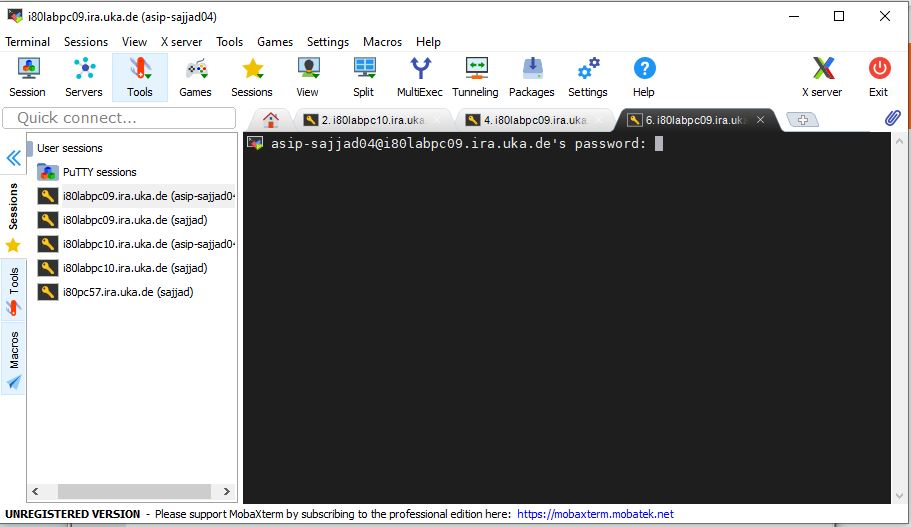
\includegraphics[width=5.67963in,height=3.28535in]{images/media/image16.JPG}

Figure 16: Logging in and Requiring Password

\begin{enumerate}
\def\labelenumi{\arabic{enumi}.}
\setcounter{enumi}{6}
\item
  You are now logged into the lab PC using MobaXterm.
\end{enumerate}

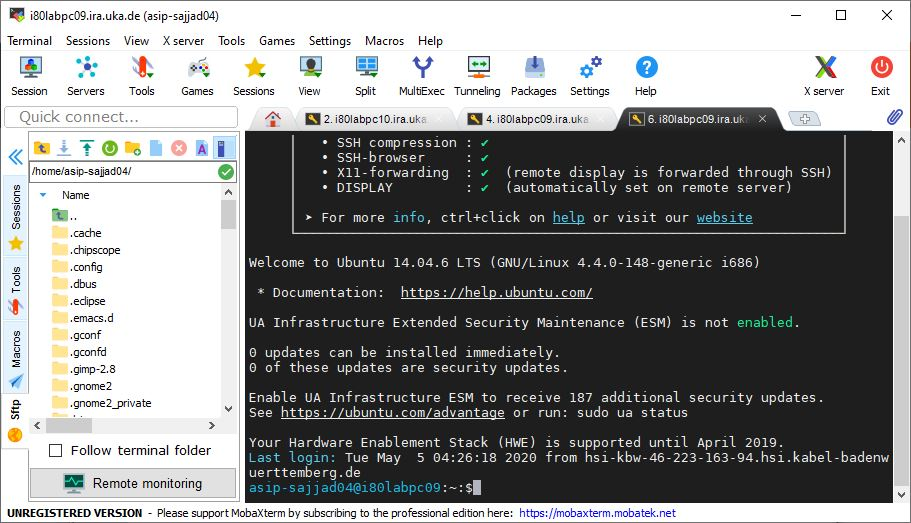
\includegraphics[width=5.70556in,height=3.27527in]{images/media/image17.JPG}

Figure 17: Logged into Remote PC

\begin{enumerate}
\def\labelenumi{\Alph{enumi}.}
\setcounter{enumi}{8}
\item
  \textbf{Recommended Practice.}
\end{enumerate}

\begin{enumerate}
\def\labelenumi{\arabic{enumi}.}
\setcounter{enumi}{7}
\item
  It is \textbf{recommended} to log into \textbf{i80pc57} as this PC
  contains the ASIPmeister software. Try to perform lab on this PC. Use
  \textbf{i80labpc10} when you need to implement your applications on
  FPGA.
\item
  To repeatedly login to some PC and avoid password, use DSA-keys and
  copy to desired PC.
\item
  Type "\textbf{ssh-keygen -t dsa}" and press Enter. Leave the default
  options. Leave the password empty.
\end{enumerate}

asip-sajjad04@i80labpc09:\textasciitilde:\$ssh-keygen -t dsa

Generating public/private dsa key pair.

Enter file in which to save the key (/home/asip-sajjad04/.ssh/id\_dsa):

/home/asip-sajjad04/.ssh/id\_dsa already exists.

Overwrite (y/n)? y

Enter passphrase (empty for no passphrase):

Enter same passphrase again:

Your identification has been saved in /home/asip-sajjad04/.ssh/id\_dsa.

Your public key has been saved in /home/asip-sajjad04/.ssh/id\_dsa.pub.

The key fingerprint is:

af:c3:84:62:4e:f4:e6:5e:cb:d1:03:19:ff:63:a9:ad asip-sajjad04@i80labpc09

The key's randomart image is:

+-\/-{[} DSA 1024{]}-\/-\/-\/-+

\textbar{} \textbar{}

\textbar{} \textbar{}

\textbar{} . \textbar{}

\textbar{} . + \textbar{}

\textbar{} . . .S . \textbar{}

\textbar{} + + .+ . . \textbar{}

\textbar{} + + oo + = \textbar{}

\textbar{} . .oo+ = . \textbar{}

\textbar{} .. +.E.. \textbar{}

+-\/-\/-\/-\/-\/-\/-\/-\/-\/-\/-\/-\/-\/-\/-\/-\/-+

\begin{enumerate}
\def\labelenumi{\arabic{enumi}.}
\setcounter{enumi}{10}
\item
  Then copy this generated DSA-key to desired PC by type following
  command and enter your password.
\end{enumerate}

asip-sajjad04@i80labpc09:\textasciitilde:\$ssh-copy-id -i
\textasciitilde/.ssh/id\_dsa.pub asip-sajjad04@i80pc57

/usr/bin/ssh-copy-id: INFO: attempting to log in with the new key(s), to
filter out any that are already installed

/usr/bin/ssh-copy-id: INFO: 1 key(s) remain to be installed -\/- if you
are prompted now it is to install the new keys

asip-sajjad04@i80pc57's password:

Number of key(s) added: 1

Now try logging into the machine, with: "ssh 'asip-sajjad04@i80pc57'"

and check to make sure that only the key(s) you wanted were added.

\begin{enumerate}
\def\labelenumi{\arabic{enumi}.}
\setcounter{enumi}{11}
\item
  Now log into i80pc57 using ``ssh -X'' it will ask for the password.
\end{enumerate}

asip-sajjad04@i80labpc09:\textasciitilde:\$ssh -X i80pc57

Last login: Wed May 6 05:11:07 2020 from i80labpc09.irf.uni-karlsruhe.de

asip-sajjad04@i80pc57:\textasciitilde:\$

\begin{enumerate}
\def\labelenumi{\Alph{enumi}.}
\setcounter{enumi}{9}
\item
  \textbf{Setting up .bashrc.user}
\end{enumerate}

\begin{enumerate}
\def\labelenumi{\arabic{enumi}.}
\setcounter{enumi}{12}
\item
  Whenever you are logged into any PC, this file is executed at the
  login. Please set different variables in this file carefully. Usually
  the following variables should be like this:
\end{enumerate}

asip-sajjad04@i80pc57:\textasciitilde:\$cat .bashrc.user

export ASIPS\_LICENSE=29000@i80asip.ira.uka.de

export PATH=/AM/ASIPmeister/bin:\$PATH

export ASIP\_APDEV\_SRCROOT=/home/asip00/epp/AM\_tools

export PATH=/usr/java/jre1.6.0\_45/bin:\$PATH

export ASIPmeister\_Home=/AM/ASIPmeister

export ASIPmeister\_HOME=/AM/ASIPmeister

. /home/adm/modelsim\_66d.setup

. /home/adm/xilinx\_13.2\_32bit.setup

asip-sajjad04@i80pc57:\textasciitilde:\$
\section{First argument}
In this section we speak about the first argument: the rings \index{rings} around Neptune. 
bla bla bla bla blablablabla blabla bla blabla blablablabla blabla bla blabla blablablabla blabla bla blabla blablablabla blabla bla bla
bla bla bla
bla bla bl
bla bla bla
bla bla bla bl
bla bla bla b
bla bla bla 
bla bla bla bla blablablabla blabla bla bla
bla bla bla bla blablablabla blabla bla bla
\begin{figure}[!h]
\begin{center}

\includegraphics[width=0.5\textwidth]{images/section1/neptune}
\end{center}
\caption{Rings on Neptune\index{Neptune} (not only on Saturn). \label{fig:neptune}}
\end{figure}
bla bla bla bla blablablabla blabla bla bla
bla bla bla bla blablablabla blabla bla bla
bla bla bla bla blablablabla blabla bla bla
bla bla bla bla blablablabla blabla bla bla
bla bla bla bla blablablabla blabla bla bla
bla bla bla bla blablablabla blabla bla bla
bla bla bla bla blablablabla blabla bla bla
bla bla bla bla blablablabla blabla bla bla
bla bla bla bla blablablabla blabla bla bla

\section{Second argument}
In this section we speak about the second argument: and now for something completely different (cit. Monty Python\index{Monty Python} \cite{MontyPython})

\section{Third argument}
In this section we speak about the third and last argument: the meaning of life. 
The answer \cite{Hitchhikers} to the question of the sense of life, the universe and everything is very well known: 42.
The problem is how to formulate the question in such a way that we can understand the answer.  


\printbibliography
\printindex


\end{document}

